\section{Results}


In this Section, the \Dstar roduction cross sections are shown in Fig.~\ref{fig:DmesonCorrYields}. Figure~\ref{fig:DmesonCorrYieldsCompar} shows the comparison between the new analysis with full pp sample collected in 2016, 2017 and 2018 with respect to the old analysis only with data sample collected in 2016. The $\pt$-differential cross section of prompt \Dstar is compared to theoretical model, FONLL, is shown in Fig.~\ref{fig:DmesonCorrYieldsModel}.


\begin{figure}[tb]
\begin{center}
%\includegraphics[width=0.48\textwidth]{PlotsRAA/Dzero_dNdpt_010_3050.pdf}
%\includegraphics[width=0.48\textwidth]{PlotsRAA/Dplus_dNdpt_010_3050.pdf}
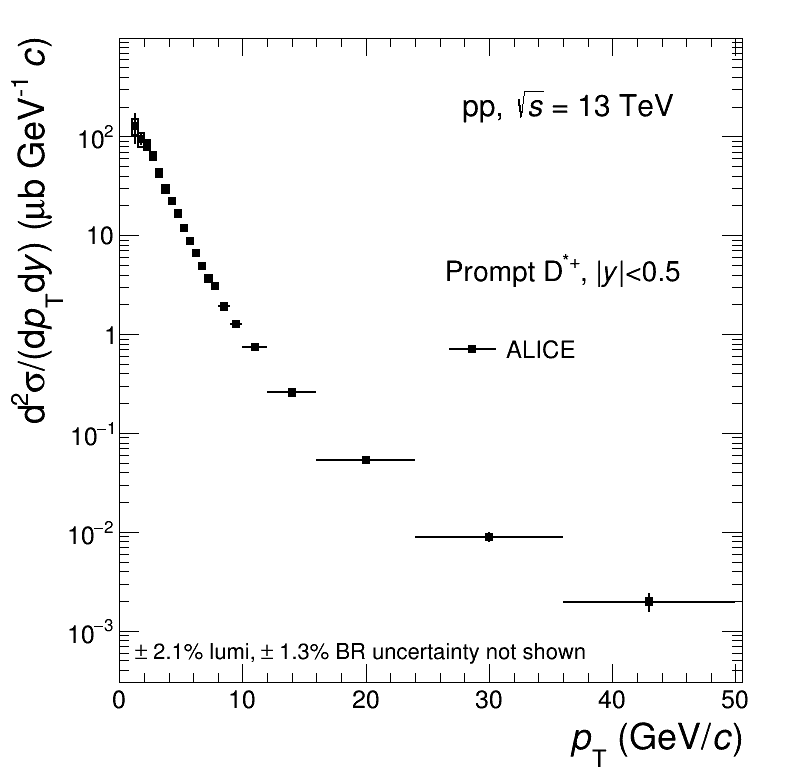
\includegraphics[width=0.55\textwidth]{figures/Dstar/pp13TeV/cross-setion-pp13TeV.png}
%\includegraphics[width=0.48\textwidth]{PlotsRAA/Ds_dNdpt_010_3050.pdf}
\caption{$\pt$-differential inclusive production cross section of prompt \Dstar mesons in pp collisions at \s 13 TeV.} 
% pT -differential inclusive production cross section of prompt
\label{fig:DmesonCorrYields}
\end{center}
\end{figure}



\begin{figure}[tb]
\begin{center}
%\includegraphics[width=0.48\textwidth]{PlotsRAA/Dzero_dNdpt_010_3050.pdf}
%\includegraphics[width=0.48\textwidth]{PlotsRAA/Dplus_dNdpt_010_3050.pdf}
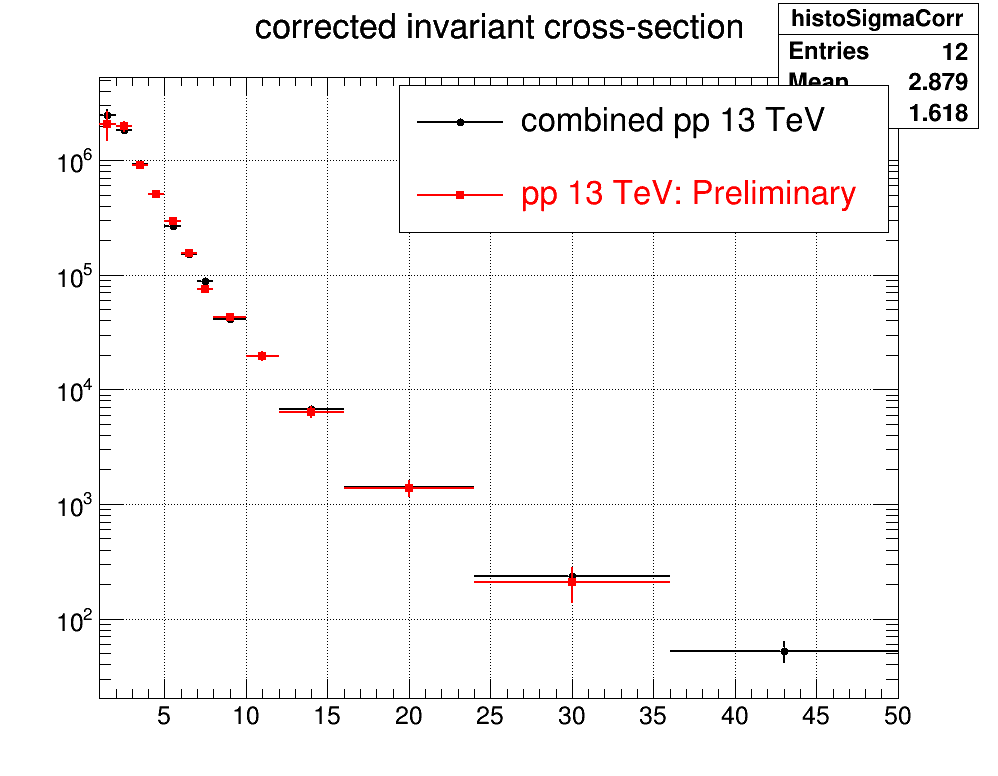
\includegraphics[width=0.65\textwidth]{figures/Dstar/pp13TeV/comparison_plt_dstar.png}
%\includegraphics[width=0.48\textwidth]{PlotsRAA/Ds_dNdpt_010_3050.pdf}
\caption{Comparison new analysis full data sample (2016, 2017 and 2018) with respect to the only 2016 data in pp collisions at \s 13 TeV.} 
% pT -differential inclusive production cross section of prompt
\label{fig:DmesonCorrYieldsCompar}
\end{center}
\end{figure}


\begin{figure}[tb]
\begin{center}
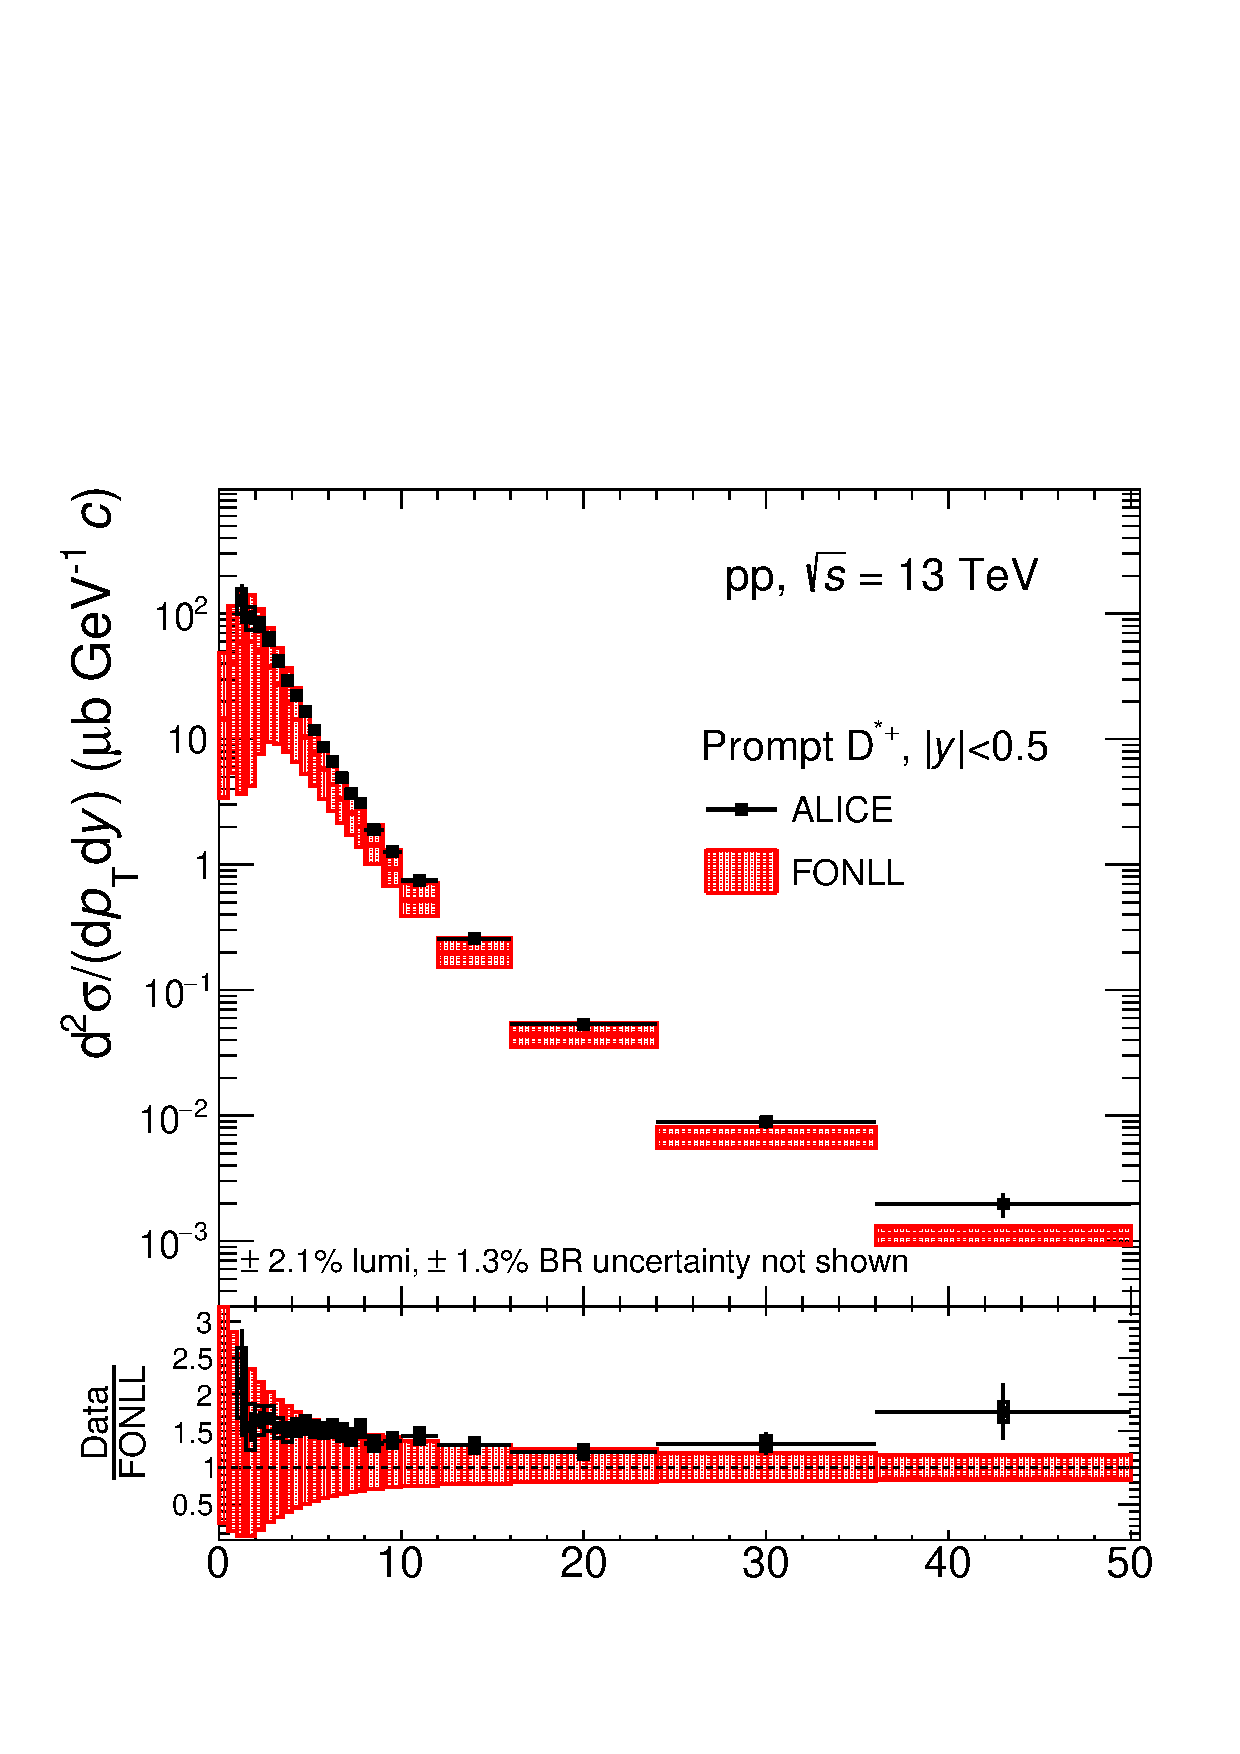
\includegraphics[width=1\textwidth]{figures/Dstar/pp13TeV/cross-section-pp13TeV-final-systematics.pdf}
\caption{$\pt$-differential inclusive production cross section of prompt \Dstar mesons in pp collisions at \s 13 TeV compared with FONLL.}
\label{fig:DmesonCorrYieldsModel}
\end{center}
\end{figure}
